\section{Kommunikation}

\subsection{Client $\leftrightarrow$ Server} 
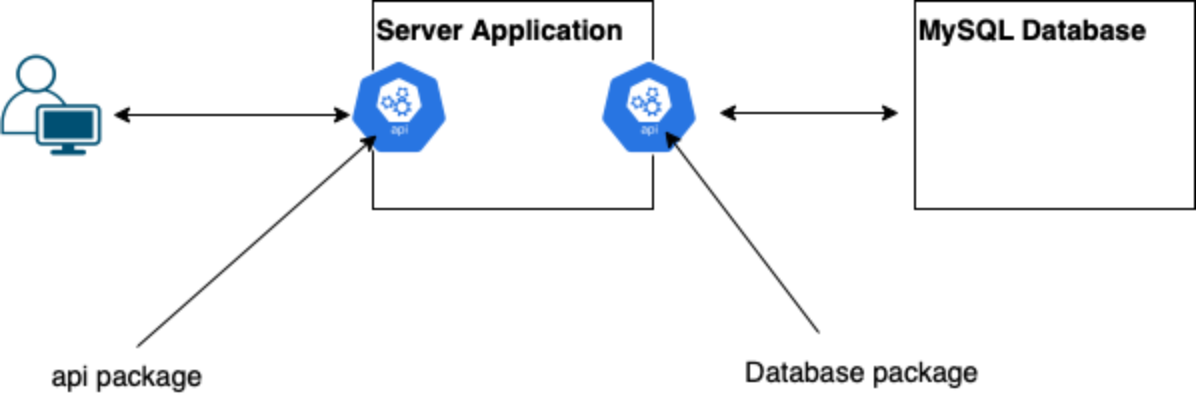
\includegraphics[width=1\textwidth]{res/Kommunikation.png}
Die Kommunikation zwischen Client und Server erfolgt über das \nameref{API}, bei der die Klasse FrontendAPI 
als RESTful API über JSON mit dem Client kommuniziert und das Database Package die Kommunikation 
zwischen der Datenbank und der Server Application regelt. Beide Schnittstellen sind zugleich Fassaden, die die Kommunikation
zwischen den einzelnen Subsystemen regeln.
Hier ist also eine horizontale Schichtenarchitektur vorhanden.

%Frontend API
\subsubsection{Frontend API}
Hinweis: Json Objekte werden in Python nativ als String interpretiert. Das ist dementsprechend im Entwurf aber durch die 
Benennung der Parameter klar, da json Objekte immer mit json\texttt{\_}details o.Ä. beschrieben werden. \\ \\
Mithilfe von Flask läuft auf dem Hostserver eine RESTful API, von der ein Status Code geholt werden kann, der über den Erfolg 
bzw. über den Art des geworfenen Fehlers Auskunft gibt.\\ 
Da wir uns hier mit Fehlern der MatFlow Anwendung auseinandersetzen, sind alle Fehler im 6xx Format.
Folgende spezifische Fehlerarten gibt es, d.h. diese Status Codes erweitern die standardisierten Codes wie etwa 404:
\begin{itemize}
    \item 601: UserExistsException
    \item 602: DoubleTemplateNameException
    \item 603: InvalidDagFileException
    \item 604: DoubleWorkflowInstanceNameException
    \item 605: EmptyConfigFolderException
    \item 606: WorkflowInstanceRunningException
    \item 607: successful Operation
\end{itemize}

%Lukas zum Database package
\subsubsection{Database package}
Die Kommunikation zwischen BackEnd und MySQL-Server läuft allein durch die Klasse DatabaseTable des Pakets \nameref{database}. 
Der Verbindungsaufbau ist mit der Pythonbibliothek MySQLdb vorgesehen.


\subsection{Server $\leftrightarrow$ Airflow API}
Der Server kommuniziert mit Airflow über die Airflow API, um die Benutzerrollen Reviewer, Developer und Administrator zu erstellen.
Außerdem wird die Airflow API dazu benötigt, Benutzer zu registrieren und zu bearbeiten.
Des Weiteren wird die Airflow API dazu benutzt um herauszufinden ob ein bestimmter Workflow gerade ausgeführt wird.

\newpage